\documentclass[12pt]{article}
\usepackage{enumitem}
\usepackage{graphicx}
\begin{document}
\section*{\center LATEX assignment}
\begin{enumerate}
    \item  The ratio of HCF to LCM of the least composite number and the least prime number is :
    \begin{enumerate}[label=(\alph*)]
      \item 1:2
      \item 2:1
      \item 1:1
      \item 1:3
    \end{enumerate}
    \item The next term of the A.P.: $\sqrt{7}$, $\sqrt{28}$, $\sqrt{63}$ is :
    \begin{enumerate}[label=(\alph*)]
      \item $\sqrt{70}$
      \item $\sqrt{80}$
      \item $\sqrt{97}$
      \item $\sqrt{112}$
    \end{enumerate}
    \item Two numbers are in the ratio 2 : 3 and their LCM is 180. what is the HCF of these numbers ?
    \item \begin{enumerate}[label=(\Alph*)]
    \item How many terms are there in A.P whose first and fifth term are - 14 and 2, respectively and the last term is 62.
\begin{center}
   \textbf{OR}
\end{center}
\item Which term of the A.P.:65, 61, 57, 53, ................ is the first negative term ?
    \end{enumerate}
    \item Prove that $\sqrt{5}$ is an irrational number.
    \item If \lq p\rq and \lq q\rq are natural numbers and \lq p\rq is the multiple of \lq q\rq, then what is the HCF of \lq p\rq and \lq q\rq ?
    \begin{enumerate}[label=(\alph*)]
      \item pq
      \item p
      \item q
      \item $p+q$
      \end{enumerate}
    \item Prove that $2+\sqrt{3}$ is an irrational number, given that $\sqrt{3}$ is an irrational number.
    \item\begin{enumerate}[label=(\Alph*)]
        \item Find by prime factorisation the LCM of the numbers $18180$ and $7575$. Also, find the HCF of the two numbers
        \begin{center}
            \textbf{OR}
        \end{center}
        \item Three bells ring at intervals of 6, 12 and 18 minutes. If all the three bells rang at 6 a.m., when will they ring together again ?
        \end{enumerate}
    \item How many terms of the arithmetic progression 45, 39, 33, ...... must be taken so that their sum is 180 ? Explain the double answer.
    \item If $p-1$, $p+1$ and $2p+3$ are in A.P., then the value of $p$ is
        \begin{enumerate}[label=(\alph*)]
      \item -2
      \item 4
      \item 0
      \item 2
      \end{enumerate}
    \item Assertion (A): The perimeter of$\Delta$ABC is a rational number.\\Reason (R): The sum of the squares of two rational numbers is always rational.
    \begin{center}
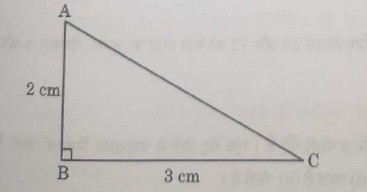
\includegraphics[width=5cm, height=4cm]{/sdcard/internship/images/30_1_1_20.png}
     \end{center}
    \item Find the greatest number which divides 85 and 72 leaving remainders 1 and 2 respectively.
    \item Prove that $\sqrt{5}$ is an irrational number.
    \item \begin{enumerate}[label=(\Alph*)]
        \item The ratio of the 11\textsuperscript{th} term to 17\textsuperscript{th} term of an A.P. is $3:4$. Find the ratio of 5\textsuperscript{th} to 21\textsuperscript{th} of the same A.P. Also, find the ratio of the sum of first 5 terms to that of first 21 terms
        \begin{center}
            \textbf{OR}
        \end{center}
        \item $250$ logs are stacked in the following manner:\\
        22 logs in the bottom row , 21 in the next row, 20 in the row next to it and so on(as shown by an example). In how many, are the 250 logs placed and how many logs are there in top row ?
         \begin{center}
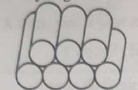
\includegraphics[width=5cm, height=4cm]{/sdcard/internship/images/30_1_1_35.png}
     \end{center}
    \end{enumerate}
\end{enumerate}
\end{document}
